%% josis.tex 1.4   2016-09-15    JoSIS latex template
%------------------------------------------------------------------
% Filename: josis_template.tex
%
% This file is intended as a template for typesetting articles for the
%
%                        Journal of Spatial Information Science.
%
% Please edit this template to generate your own formatted manuscripts
% for submission to JOSIS. See http://josis.org for further details.
%


%%% JOSIS checks in typesetting
%%% * All titles and sections lower case *EXCEPT short title  [ ]
%%% * Remove author postal addresses, only have geographic places and institutions [ ] 
%%% * Consistent use of Section, Figure, Table (capitalized and in full) [ ]
%%% * 10 keywords (and all lower case) [ ]
%%% * Remove all avoidable footnotes [ ]
%%% * Use double quotation marks (``'' not "" or `') [ ]
%%% * Punctuation inside quotations [ ]
%%% * E.g. and i.e. followed by comma [ ]
%%% * cf. followed by tilde [ ]
%%% * Itemize and enumerate correctly punctuated [e.g., "1. x, 2. y, and 3. x." ]
%%% * And/or lists using American English punctuation (e.g., "x, y, and z") [ ] 
%%% * Bibliography (e.g., en-dashes for number ranges, consistent "Proc.~" for Proceedings of..., etc.) []
%%% * Acknowledgment style use section* [ ] 
%%% * et al. no italics, but with dot  [ ] 
%%% * All captions end with full stop  [ ] 
%%% * Table captions under, not over table  [ ]
%%% * Adjust urls with burlalt [ ] 
%%% * Check correct use of hyphens, emdashes, endashes  [ ]
%%% * Perform spell check  [ ] 

%%% JOSIS checks directly before publication 
%%% Check DOI, page numbers on article and web site. [ ]
%%% Update web site with final title, abstract, keywords. [ ] 
%%% Build with distiller for DOI links. [ ]


% Required documentclass definition for JOSIS
\documentclass{josis}
\usepackage{hyperref}
\usepackage[hyphenbreaks]{breakurl}
\usepackage{booktabs}
\usepackage{stmaryrd}
\usepackage[T1]{fontenc}
\usepackage{cite}
\usepackage{subcaption}
\documentclass{article}
\usepackage{graphicx}
\usepackage{caption}
\usepackage{subcaption}
% Suggested packages for algorithm formatting
\usepackage{algorithm}
%\usepackage{algorithmic}
\usepackage{algpseudocode}
\usepackage{pythonhighlight}
\usepackage{placeins}
\usepackage{amssymb,amsmath}
%\usepackage[table]{xcolor}
\usepackage{lastpage}
\renewcommand{\topfraction}{0.9} 
\renewcommand{\textfraction}{0.1}
% Page setup and overhangs
\sloppy
\widowpenalty=10000
\clubpenalty=10000
\hyphenpenalty=75

% Article details for accepted manuscripts will be added by editorial staff
% Omit year if article in press
% Omit number if article under review
\josisdetails{%
   number=2, year=2024, firstpage=1, lastpage=\pageref{LastPage}, 
  doi={CodeCadets},
  % received={December 24, 2015}, 
   %returned={February 25, 2016},
   %revised={July 13, 2016},
   %accepted={September 5, 2016},
   }

%\newcommand{\mydoi}[1]{\href{http://dx.doi.org/#1}{doi:\protect\detokenize{#1}}}

%\renewcommand{\UrlLeft}{http:\sslash}
%\DeclareUrlCommand\myurl{\def\UrlLeft{}\def\UrlRight{}%
%\urlstyle{tt}}

\urlstyle{rm}
\makeatletter
% Inspired by http://anti.teamidiot.de/nei/2009/09/latex_url_slash_spacingkerning/
% but slightly less kern and shorter underscore
\let\UrlSpecialsOld\UrlSpecials
\def\UrlSpecials{\UrlSpecialsOld\do\/{\Url@slash}\do\_{\Url@underscore}}%
\def\Url@slash{\@ifnextchar/{\kern-.11em\mathchar47\kern-.2em}%
    {\kern-.0em\mathchar47\kern-.08em\penalty\UrlBigBreakPenalty}}
\def\Url@underscore{\nfss@text{\leavevmode \kern.06em\vbox{\hrule\@width.3em}}}
\makeatother

\hypersetup{
colorlinks=true,
linkcolor=black,
citecolor=black,
urlcolor=black
} 

% Add the running author and running title information
\runningauthor{\begin{minipage}{.9\textwidth}\centering Hemal Shaji,Leya Kurian,Mayakha Sara Saji,Neenu Ann Varghese,Swathy Mahesh \end{minipage}}
\runningtitle{Running GenAI on Intel Laptops \& Simple LLM Inference on CPU \& fine-tuning of LLM Models \texttt{openVino}}

% Document begins
\begin{document}
%\setcounter{page}{33}


% Insert your own title
\title{Running GenAI on Intel AI Laptops and Simple LLM Inference on CPU and fine-tuning of LLM Models using Intel \texttt{openVino}}

% Insert your manuscipts authors, affiliations, and addresses
\author{Hemal Shaji}
\author{Leya Kurian}
\author{Mayakha Sara Saji }
\author{Neenu Ann Varghese}
\author{Swathy Mahesh}\affil{Saintgits Group of Institutions, Kottayam, Kerala}
\date{}
\maketitle
% Add 5-10 keywords for every submission
\keywords{Generative Artificial Intelligence, GenAI, Intel AI Laptops, Large Language Models, LLM Inference, CPU Optimization, \texttt{openVino}, Fine-tuning, Performance Benchmarking, Documentation}
% Add a short abstract of 150-250 words 
\begin{abstract}
This project investigates the deployment of Generative Artificial Intelligence (GenAI) on Intel AI laptops, focusing on the efficiency and practicality of running Large Language Model (LLM) inference on CPUs. It also explores the fine-tuning of these models using Intel's \texttt{openVino} toolkit. The project includes benchmarking performance, optimizing CPU usage for LLM inference, and implementing a streamlined process for fine-tuning models. The solution comprises a detailed performance analysis, an optimization guide, and thorough documentation, aiming to enhance the practical understanding of GenAI applications on Intel hardware. 
\end{abstract}
% Your main text begins here. 
\section{Introduction}
The advent of Generative Artificial Intelligence (GenAI) has revolutionized various fields, including natural language processing and creative content generation. Traditionally, deploying these advanced models has required significant computational resources, often provided by powerful GPUs. This report explores a more accessible and cost-effective approach by leveraging Intel AI laptops and their CPUs for GenAI tasks.

Intel AI laptops, with their robust processing capabilities optimized for AI workloads, present a promising platform for running Large Language Model (LLM) inference. Efficient execution of LLM tasks on CPUs can democratize access to GenAI, making it feasible for a broader range of applications and users. This project evaluates the performance of Intel AI laptops in this context and seeks to optimize CPU usage for effective LLM inference.

Additionally, fine-tuning LLM models is crucial for tailoring them to specific tasks and enhancing their performance. Intel's \texttt{openVino} toolkit offers a suite of tools designed to accelerate deep learning inference on Intel hardware. This report delves into the process of fine-tuning LLMs using \texttt{openVino}, providing insights into its advantages and practical implementation strategies.

The project also explores advanced applications of GenAI, including the development and optimization of open-domain chatbots. Effective conversation in chatbots requires skills such as engaging talking points, listening, asking and answering questions, and displaying knowledge, empathy, and personality appropriately. By leveraging Intel's \texttt{openVino} toolkit, we aim to enhance these capabilities in large-scale models.

Through comprehensive analysis, benchmarking, and practical experimentation, this report aims to enhance the understanding of deploying GenAI on Intel AI laptops, offering valuable guidance for developers and researchers in harnessing GenAI's potential on accessible hardware platforms.
\section{Literature Review}
The paper by Demidovskij et al. (2020) discusses the \texttt{openVino} toolkit, focusing on the features and capabilities of the \texttt{openVino} Deep Learning Workbench, a platform designed to help developers optimize, analyze, and deploy deep learning models. The authors cover aspects such as performance improvements, ease of use, supported functionalities, and practical applications of the toolkit in real-world AI deployments \cite{Demidovskij2020}.

Jeong (2023) explores the implementation of generative AI services by leveraging a large language model (LLM) application architecture that is based on enterprise data. This study addresses challenges such as data management, system architecture, and practical applications within a business context, providing insights and methodologies for utilizing LLMs effectively in enterprise environments to enhance service capabilities \cite{Jeong2023}.

McIntosh et al. (2024) critically examine the limitations of current benchmarks for evaluating large language models (LLMs) amidst the advancements in generative AI. They highlight how these benchmarks fail to capture the full spectrum of LLM capabilities and limitations, potentially leading to an incomplete or skewed understanding of their performance. The authors propose the need for more comprehensive and adaptive benchmarking methodologies \cite{McIntosh2024}.

Mo et al. (2024) address the challenge of detecting AI-generated text produced by large language models. They propose a detection method leveraging transformer-based deep learning algorithms to distinguish between human-written and AI-generated text. The study details the design and implementation of their detection algorithm, including the architecture of the transformer model, training procedures, and evaluation metrics. Experimental results demonstrate the effectiveness of their approach in identifying AI-generated content across various datasets \cite{Mo2024}.

Maurya et al. (2024) introduce a novel checkpointing mechanism tailored for large language models (LLMs). The proposed method, DataStates-LLM, employs lazy asynchronous checkpointing to efficiently manage the state of LLMs during training and inference. This technique aims to reduce the overhead and performance bottlenecks associated with traditional synchronous checkpointing by deferring checkpoint operations and asynchronously writing them to storage. The authors demonstrate that DataStates-LLM significantly improves the efficiency and reliability of LLM training processes \cite{Maurya2024}.

\section{Methodology}
\begin{itemize}
    \item \textbf{\texttt{openVino} Toolkit:} \texttt{openVino} (Open Visual Inference and Neural Network Optimization) is utilized to optimize and deploy deep learning models on Intel hardware. It provides tools to convert models to \texttt{openVino} IR format and enables efficient inference, making it a crucial component for model optimization and deployment in our project.

    \item \textbf{PyTorch Library:} PyTorch is an open-source machine learning library widely used for developing and training deep learning models. It is used to load the Blenderbot model and perform the initial model conversion to ONNX format due to its flexible and user-friendly interface.

    \item \textbf{Transformers Library:} The Transformers library by Hugging Face is employed to handle various tasks related to Natural Language Processing (NLP). It provides pre-trained models and tokenizers, which are used for loading and preparing the Blenderbot model for conversion.

    \item \textbf{ONNX (Open Neural Network Exchange):} ONNX is an open format for AI models, enabling interoperability between different frameworks. The model is converted from PyTorch to ONNX format to facilitate further conversion to \texttt{openVino} IR format, which is necessary for efficient inference on Intel hardware.

    \item \textbf{NNCF (Neural Network Compression Framework):} NNCF is used for quantizing the model. It provides utilities to apply quantization techniques, which reduce the model size and improve inference speed without significant loss in accuracy. This step is critical for optimizing the model for deployment in resource-constrained environments like Intel AI laptops.

    \item \textbf{Integrated Development Environment (IDE):} An IDE like Visual Studio Code is used to streamline the development process. It provides tools for writing, testing, and debugging code, enhancing productivity and collaboration among team members.

    \item \textbf{Version Control System (Git):} Git is employed to manage the project's source code, track changes, and facilitate collaboration. It ensures that code can be safely modified and maintained, with a history of changes that can be referenced or reverted if necessary.
\end{itemize}

\section{Implementation}

\subsection{User Interface}
The GUI for the GenAI project on Intel laptops is designed to be intuitive and user-friendly, ensuring seamless interaction with the AI system. Built using HTML, CSS, JavaScript, the GUI offers a dynamic and responsive interface. It comprises various interactive elements such as buttons, menus, and dialogs, facilitating easy navigation and operation. The architecture follows a modular design, where the user interface communicates with the GenAI engine through a dedicated controller. This separation ensures maintainability and scalability, allowing the GUI to be extended or modified independently of the core AI functionalities.
\begin{figure}[h]
    \centering
    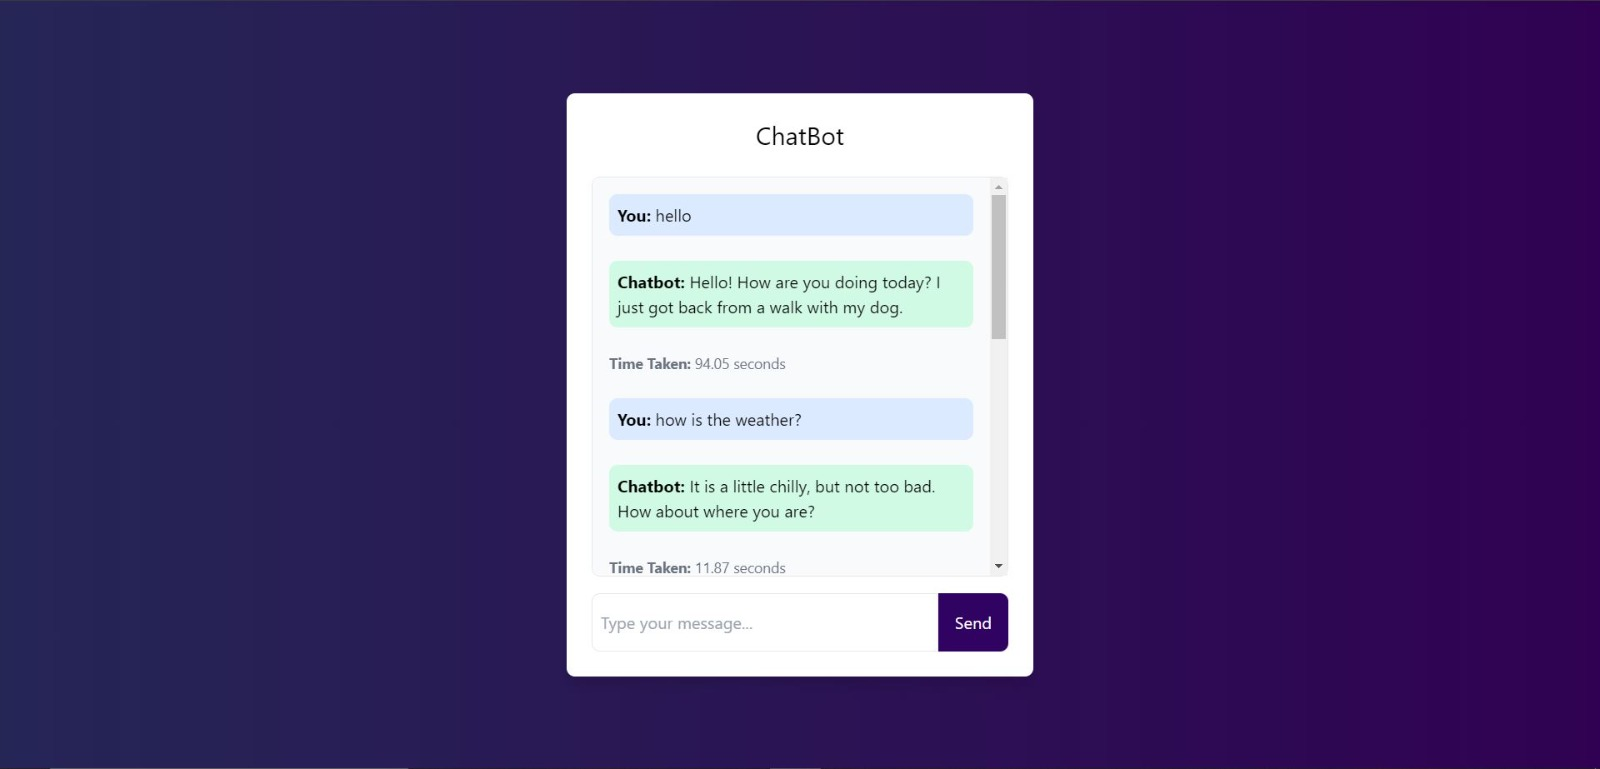
\includegraphics[width=\textwidth]{gui.jpg}
    \caption{User Interface}
    \label{fig:chatbot_implementation}
\end{figure}
\subsection{Model Development}
In the chatbot development project, the team initially utilized the GPT-2 model, which generated largely nonsensical outputs. To address this issue, the team adopted the Blenderbot400M Distill model, resulting in significantly improved performance compared to GPT-2. Despite observing a slight degradation in model accuracy post-quantization, the performance of Blenderbot400M Distill remained acceptable.

In an effort to further enhance performance, the team experimented with the Blenderbot9B model. However, due to disk space constraints on the system, the conversion to the ONNX format was not feasible, although it was successful on Google Colab. Consequently, the decision was made to proceed with Blenderbot400M Distill as the final choice for the chatbot development. 

\subsection{Model Optimization}

The process of optimizing the Blenderbot model involves several key steps to prepare the model for deployment using \texttt{openVino} and NNCF for quantization. Below is a detailed description of each step involved in the model optimization process:

\begin{enumerate}
    \item \textbf{Install Necessary Packages:} The required Python packages include `\texttt{openVino}`, `optimum[\texttt{openVino}]`, `nncf`, `transformers`, and `torch`. These packages are essential for model conversion and quantization.

    \item \textbf{Download and Convert the Model:} The Blenderbot model and its tokenizer are downloaded from the Hugging Face library. An example input is tokenized, and the model is exported to the ONNX format. The output directory and file paths are specified to store the ONNX model.

    \item \textbf{Convert ONNX Model to \texttt{openVino} IR Format:} The ONNX model is loaded using the \texttt{openVino} core. The model is then serialized to the \texttt{openVino} Intermediate Representation (IR) format, saving the model in XML and BIN files.

    \item \textbf{Create Dummy Calibration Dataset:} A dummy calibration dataset is created to simulate real data for quantization purposes. This dataset includes random tensor data that matches the input shape expected by the model.

    \item \textbf{Quantize the Model:} Using the Neural Network Compression Framework (NNCF), the model is quantized. The NNCF configuration specifies the input shape and quantization parameters. The quantized model is saved in \texttt{openVino} format.

    \item \textbf{Save the Pretrained Model and Tokenizer Configuration:} The pretrained Blenderbot model and tokenizer configuration files are saved for later use in the pipeline.

\end{enumerate}

\subsection{Using \texttt{openVino}}
After optimizing the Blenderbot model, the next step is to implement it using \texttt{openVino} for efficient inference. Below are the detailed steps involved in this process:

\begin{enumerate}
    \item \textbf{Initialize the Pipeline with the Quantized Model:} The text-to-text generation pipeline is initialized using the quantized Blenderbot model and tokenizer. This step ensures the model is ready for inference.

    \item \textbf{Implement the Chatbot:} A chatbot function is created to interact with users. This function takes user input, generates a response using the text generation pipeline, and displays the output.

\end{enumerate}

These steps collectively enhance the model's performance and efficiency, making it suitable for deployment in real-world applications.


\section{Results and Discussion}
\subsection{Quantized Model Initialization and Chatbot Implementation}

The following figures illustrate the initialization of the quantized model and the implementation of the chatbot.

\begin{figure}[h]
    \centering
    %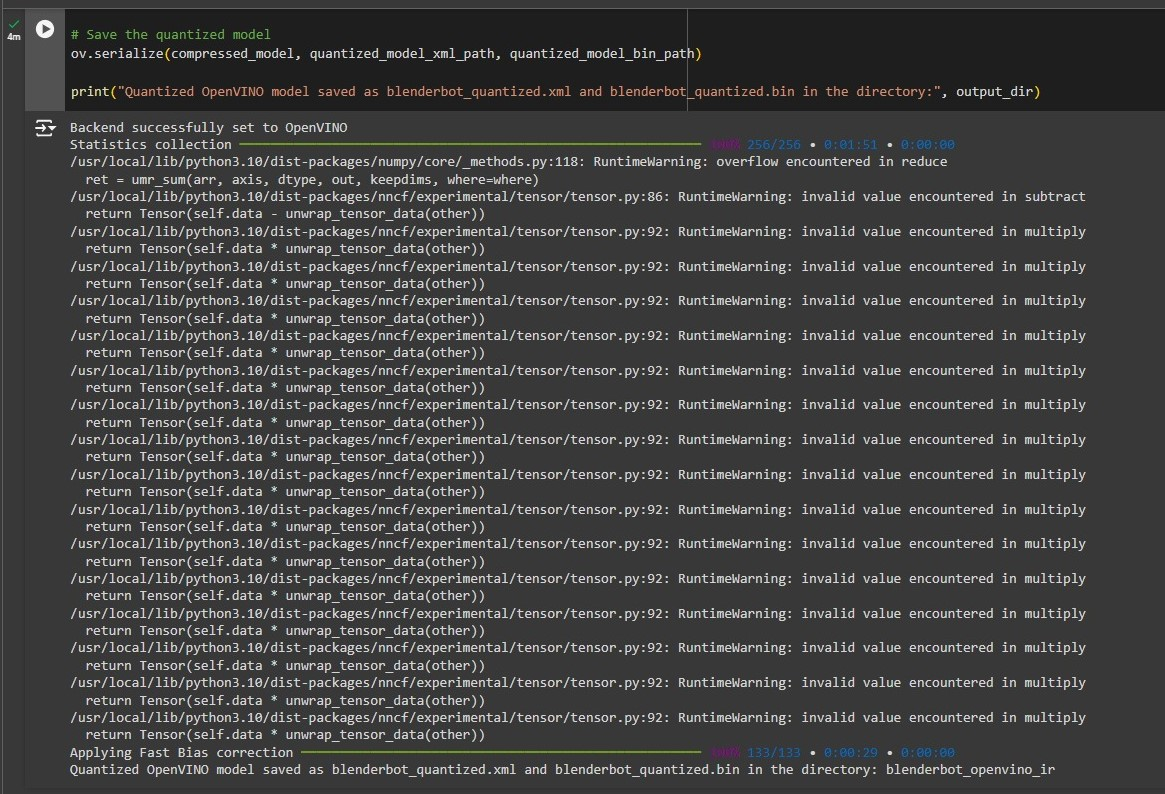
\includegraphics[width=\textwidth]{1i.jpg}
    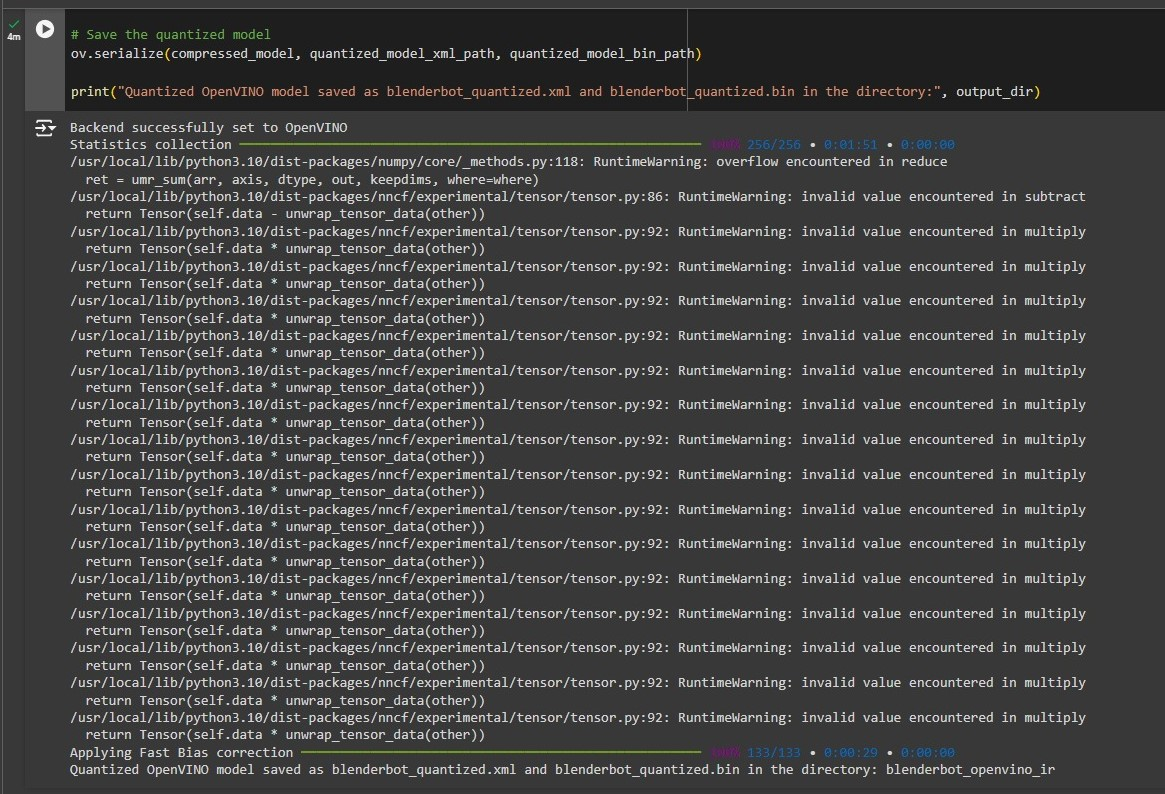
\includegraphics[scale=0.38]{1i.jpg}
    \caption{Initialization of the pipeline with the quantized model and implementation of the chatbot.}
    \label{fig:chatbot_implementation}
\end{figure}


\FloatBarrier
\subsection{Quantized Model Output}
The output of the quantized model is shown in the figure below. Despite some runtime warnings, the model was successfully quantized and saved.

\begin{figure}[H]
    \centering
    %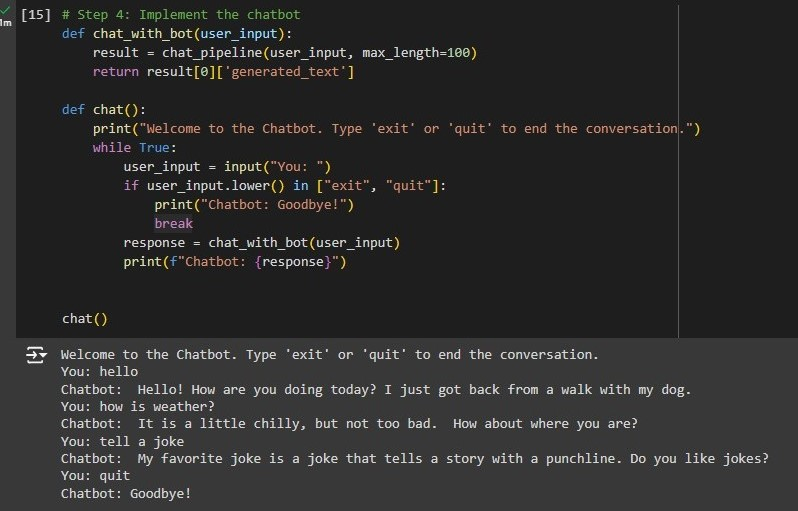
\includegraphics[width=\textwidth]{2i.jpg}
    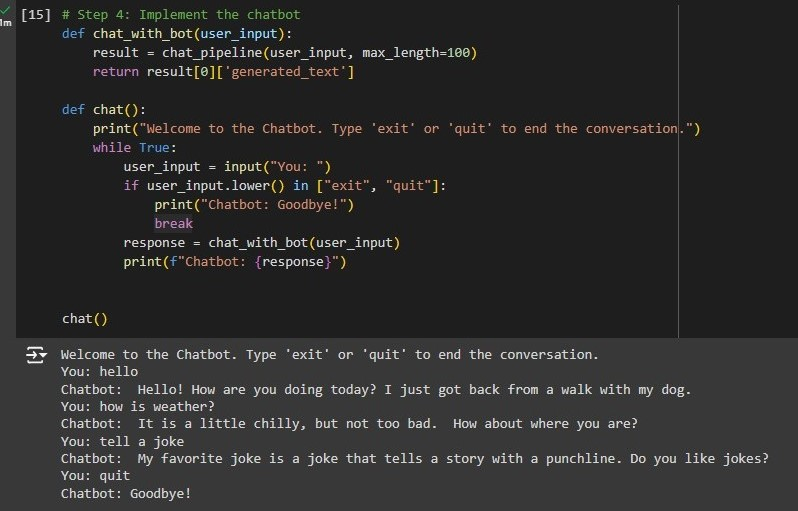
\includegraphics[scale=0.5]{2i.jpg}
    \caption{Output of the quantized model showing successful quantization despite runtime warnings.}
    \label{fig:quantized_model_output}
\end{figure}

As observed, the quantized model was successfully saved as \texttt{blenderbot\_quantized.xml} and \texttt{blenderbot\_quantized.bin} in the specified directory. These files can now be used for efficient inference with reduced model size and improved performance.

\subsection{Performance Evaluation}
\begin{table}
  \centering
  \begin{tabular}{|c|c|c|c|}
    \hline
    Parameters & Base Model & ONNX Model & IR Model\\
    \hline
    Model Size & 1.46GB & 1.39GB & 359MB \\
    \hline
    Performance Time & 13 sec & 13 sec & 0.19 sec \\
    \hline
    Relevance & Acceptable & Moderately Acceptable & Contextual\\
    \hline
  \end{tabular}
  \caption{Comparison of Various Models }
  \label{tab:example_table}
\end{table}

The comparison of model parameters for the Base Model, ONNX Model, and IR Model highlights significant differences in size, performance time, and relevance. The IR Model is the smallest at 359MB, compared to the Base Model's 1.46GB and the ONNX Model's 1.39GB. Performance-wise, the IR Model is exceptionally fast, taking only 0.19 seconds, while both the Base and ONNX models take 13 seconds. However, when it comes to relevance, the IR Model, created from scratch using Blenderbot400MDistil, falls short. Its contextual relevance is lower compared to the acceptable relevance of the Base Model and the moderately acceptable relevance of the ONNX Model. Pre-trained models like Blenderbot9B by \texttt{openVino} offer better relevance and accuracy. Despite the IR Model's advantages in size and speed, it needs significant improvement in relevance to match the performance of more established models. Ready-made models by \texttt{openVino}, such as Blenderbot9B, may provide better overall performance and accuracy, making them more suitable for applications requiring high relevance and contextual accuracy.

\section{Limitations of Study}
One limitation of this study is the reliance on the pre-trained Blenderbot model, which is based on specific datasets and may not generalize well to all conversational contexts. The model's responses are highly dependent on the training data, and it may exhibit biases present in the data. Additionally, while the use of \texttt{openVino} improves inference efficiency on Intel hardware, the quantization process may lead to a minor degradation in model accuracy, affecting the quality of the chatbot's responses. Another limitation is the computational resource requirement for model conversion and quantization, which might be prohibitive for users with limited access to high-performance computing resources.Lastly, the implementation and optimization process, although streamlined with various tools, still requires a certain level of expertise in machine learning and model deployment, which could make it difficult to design and develop the model.

\section{Conclusions}
This project successfully demonstrates the implementation and optimization of a chatbot using Generative AI on Intel AI laptops. By leveraging the \texttt{openVino} toolkit, we were able to optimize the Blenderbot model for efficient inference on Intel hardware, ensuring rapid response times and improved performance. The process involved converting the model from PyTorch to ONNX format, then further to \texttt{openVino} IR format, followed by quantization using NNCF to enhance efficiency without significant loss in accuracy.

However, the study also highlights some limitations, such as the dependency on pre-trained models and the computational requirements for model optimization. Despite these challenges, the project provides a clear pathway for implementing and optimizing AI models on resource-constrained environments, paving the way for future advancements in deploying AI solutions on edge devices.

Overall, the project not only demonstrates a practical application of AI optimization techniques but also serves as a valuable guide for similar implementations. The results indicate that with the right tools and methodologies, it is feasible to run advanced AI models efficiently on everyday computing devices, opening up new possibilities for AI-driven applications in various fields.

\section{Acknowledgments}

We would like to express our heartfelt gratitude and appreciation to Intel\textsuperscript{\textcopyright} Corporation for providing an opportunity to undertake this project. First and foremost, we extend our sincere thanks to our team mentor, Siju Swamy, for his invaluable guidance and constant support throughout the project. His expertise and encouragement have been instrumental in shaping our work. We are deeply indebted to our college, Saintgits College of Engineering and Technology, for providing us with the necessary resources and sessions on machine learning, artificial intelligence, and optimization techniques. The support from our institution has been crucial in the successful completion of our project. We extend our gratitude to all the researchers, scholars, and experts in the fields of artificial intelligence, machine learning, and model optimization, whose seminal work has paved the way for our project. Finally, we acknowledge the mentors, institutional heads, and industrial mentors for their invaluable guidance and support in completing this industrial training under the Intel\textsuperscript{\textcopyright} - Unnati Programme. Their expertise and encouragement have been fundamental to our project's success.
\cite{*}
\bibliographystyle{josisacm}
\bibliography{josisexample}
\appendix

\section{Main code sections for the solution}

\subsection{Installing Necessary Packages}
\begin{python}
!pip install openvino optimum[openvino] nncf transformers torch
\end{python}

\subsection{Downloading and Converting the Model}
\begin{python}
model_name = "facebook/blenderbot-400M-distill"
tokenizer = AutoTokenizer.from_pretrained(model_name)
model = BlenderbotForConditionalGeneration.from_pretrained(model_name)

dummy_input = tokenizer("Hello, how are you?", return_tensors="pt")
dummy_attention_mask = torch.ones(dummy_input['input_ids'].shape, dtype=torch.long)
dummy_decoder_input_ids = torch.ones((1, 1), dtype=torch.long)

output_dir = "blenderbot_openvino_ir"
os.makedirs(output_dir, exist_ok=True)
output_path = os.path.join(output_dir, "blenderbot.onnx")

torch.onnx.export(
    model,
    (dummy_input['input_ids'], dummy_attention_mask, dummy_decoder_input_ids),
    output_path,
    opset_version=11,
    input_names=["input_ids", "attention_mask", "decoder_input_ids"],
    output_names=["output"]
)
\end{python}

\subsection{Loading the ONNX Model}
\begin{python}
core = ov.Core()
onnx_model = core.read_model("/content/blenderbot_openvino_ir/blenderbot.onnx")

ir_xml_path = os.path.join(output_dir, "blenderbot_ir.xml")
ir_bin_path = os.path.join(output_dir, "blenderbot_ir.bin")

ov.serialize(onnx_model, ir_xml_path, ir_bin_path)
\end{python}

\subsection{Quantizing the Model}
\begin{python}
nncf_config = NNCFConfig.from_dict({
    "input_info": {
        "sample_size": [1, 7]
    },
    "compression": {
        "algorithm": "quantization",
        "initializer": {
            "range": {
                "num_init_samples": 256
            },
            "batchnorm_adaptation": {
                "num_bn_adaptation_samples": 256
            }
        }
    }
})

class CalibrationDataset(Dataset):
    def __getitem__(self, item):
        input_ids = torch.randint(0, 100, (1, 7), dtype=torch.int32)
        attention_mask = torch.ones((1, 7), dtype=torch.int32)
        return {"input_ids": input_ids, "attention_mask": attention_mask}

calibration_dataset = CalibrationDataset(num_samples=256, batch_size=1)
compressed_model = quantize(ov_model, calibration_dataset, preset=QuantizationPreset.MIXED)

ov.serialize(compressed_model, "blenderbot_quantized.xml", "blenderbot_quantized.bin")
\end{python}

\subsection{Saving the Pretrained Model and Tokenizer Configuration}
\begin{python}
model.save_pretrained("blenderbot_openvino_ir")
tokenizer.save_pretrained("blenderbot_openvino_ir")
\end{python}

\subsection{Initializing the Pipeline and Implementing the Chatbot}
\begin{python}
chat_pipeline = pipeline("text2text-generation", model="blenderbot_openvino_ir", tokenizer="blenderbot_openvino_ir")

def chat_with_bot(user_input):
    result = chat_pipeline(user_input, max_length=100)
    return result[0]['generated_text']

def chat():
    while True:
        user_input = input("You: ")
        if user_input.lower() in ["exit", "quit"]:
            break
        response = chat_with_bot(user_input)
        print(f"Chatbot: {response}")

chat()
\end{python}

\end{document}